\documentclass{article}
\usepackage{graphicx}
\usepackage{amsmath}
\usepackage{authblk}
\usepackage[finnish]{babel}
\usepackage{graphicx}
\graphicspath{{./}{./figures/}}
\usepackage[backend=biber,style=numeric,sorting=none]{biblatex}
\bibliography{wp_fin}
\usepackage{float}
\usepackage{csquotes}
\usepackage{amsmath}
\usepackage{mathtools}
\usepackage{url}

\usepackage[acronym, toc, description,nopostdot]{glossaries}

\makeglossaries

\newglossaryentry{p2p}{name=Vertaisverkko,description={Peer-to-Peer network\\ \url{https://fi.wikipedia.org/wiki/Vertaisverkko}\\}}

\newglossaryentry{doublespend}{name=Kaksinkertainen kulutus,description={Double-spending\\ \url{https://en.wikipedia.org/wiki/Double-spending}\\}}

\newglossaryentry{tyontodiste}{name=Työntodiste,description={Proof-of-work\\ \url{https://medium.com/brandin-kirjasto/työntodisteen-anatomia-475f371696f4}\\}}

\newglossaryentry{besteffort}{name=Parhaansa mukaan,description={Best effort basis\\ \url{https://en.wikipedia.org/wiki/Best-effort_delivery}\\}}

\newglossaryentry{escrow}{name=Erityistili tiettyä tarkoitusta varten,description={Escrow\\ \url{https://pankkiasiat.fi/escrow-tili}\\}}

\newglossaryentry{privatepublickey}{name=Julkinen ja yksityinen avain,description={Public \& private key\\ \url{https://fi.wikipedia.org/wiki/Julkisen_avaimen_salaus}\\}}

\newglossaryentry{timestamp}{name=Aikaleimapalvelin,description={Timestamp server\\ \url{https://medium.com/brandin-kirjasto/21-oppituntia-2300d2f797c0}\\}}

\newglossaryentry{hash}{name=Tiiviste,description={Hash\\ \url{https://fi.wikipedia.org/wiki/Tiiviste_(tietotekniikka)}\\}}

\newglossaryentry{ip}{name=Internetin protokollaosoite,description={IP\\ \url{https://fi.wikipedia.org/wiki/IP-osoite}\\}}

\newglossaryentry{nonce}{name=Nonssi - kertakäyttöinen arvo,description={Nonce\\ \url{https://en.wikipedia.org/wiki/Cryptographic_nonce}\\}}

\newglossaryentry{gamblersruin}{name=Uhkapelaajan turmio,description={Gambler's Ruin\\ \url{https://en.wikipedia.org/wiki/Gambler's_ruin}\\}}

\newglossaryentry{randomwalk}{name=Binominaalinen satunnaiskulku,description={Binomial random walk\\ \url{https://fi.wikipedia.org/wiki/Satunnaiskulku}\\}}

\newglossaryentry{poissondistribution}{name=Poissonin jakauma,description={Poisson distribution\\ \url{https://fi.wikipedia.org/wiki/Poissonin_jakauma}\\}}

\newglossaryentry{fanout}{name=Levittäytyminen (laajalle),description={Fan-out\\ \url{https://en.wikipedia.org/wiki/Fan-out_(software)}\\}}

\newglossaryentry{konsensus}{name=Konsensusmekanismi,description={Consensus mechanism\\ \url{https://fi.wikipedia.org/wiki/Konsensus-päätöksenteko}\\}}

\begin{document}

\title{Bitcoin: Sähköinen käteisjärjestelmä vertaisverkossa}
\author[1]{\small{Satoshi Nakamoto \\\vspace{-3mm} https://bitcoin.org/en/bitcoin-paper} \\
\vspace{0mm}
\footnotesize{Suomentanut: \\ @Biocycle, Biocycle@protonmail.com \\
Yhteistyössä: @LohkoKettu \\ Aleksi Suomalainen, @locusf \\ Antti Majakivi, @Anduck \\ Niko Laamanen, @n1kofi}}
\date{}
\maketitle

\begin{abstract}
Täysin \glsdisp{p2p}{vertais}verkossa toimiva sähköinen käteinen mahdollistaa verkossa tehtävät maksut suoraan osapuolelta toiselle kulkematta rahoituslaitoksen läpi. Digitaaliset allekirjoitukset ovat osa ratkaisua, mutta tär\-keim\-mät niiden suomat edut menetetään, jos luotettua kolmatta osapuolta yhä tarvitaan estämään \glsdisp{doublespend}{kaksin}kertainen kulutus. Esitämme kaksinkertaisen kulutuksen ongelmaan ratkaisuksi \glsdisp{p2p}{vertais}verkkoa. Verkko \glsdisp{timestamp}aikaleimaa tapahtumat \glsdisp{hash}tiivistelaskemalla ne osaksi jatkuvaa tiivisteisiin perustuvien \glsdisp{tyontodiste}{työnt}odisteiden ketjua. Tätä rekisteriä ei voi muuttaa laskematta työntodisteita uudelleen. Pisin ketju toimii paitsi todisteena tapahtumien järjestyksestä, myös todisteena siitä, että ketjuun on kulutettu yhteensä eniten prosessointitehoa. Niin kauan kuin suurinta osaa prosessointitehosta säätelevät solmut, jotka eivät tee yhteistyötä keskenään hyökätäkseen verkkoa vastaan, ne pystyvät luomaan pisimmän ketjun jättäen hyökkääjät jälkeensä. Itse verkko ei vaadi kuin minimaalisen rakenteen. Verkko lähettää viestejä \glsdisp{besteffort}parhaansa mukaan (“best effort”), ja solmut voivat vapaasti poistua verkosta ja liittyä siihen uudelleen. Uudelleen liittyessään ne hyväksyvät pisimmän \glsdisp{tyontodiste}{työnt}odisteketjun todisteeksi siitä, mitä tapahtui niiden poissa ollessaan.

\end{abstract}

\section{Johdanto}
Internetissä tapahtuva kaupankäynti on sähköisten maksujen käsittelyn osalta päätynyt nojaamaan lähes yksinomaan rahoituslaitoksiin. Vaikka järjestelmä toimii riittävän hyvin useimmissa transaktioissa, se kärsii silti luottamuspohjaisen mallin luontaisista heikkouksista. Täysin peruuttamattomat transaktiot eivät ole todellisuudessa mahdollisia, sillä rahoituslaitokset eivät voi välttyä riitatilanteiden sovittelulta. Sovittelun kustannukset nostavat transaktioiden \mbox{kustannuksia}, mikä rajoittaa pienimmän mahdollisen käytännöllisen siirtotapahtuman kokoa ja poistaa pienten satunnaisten siirtojen mahdollisuuden, ja ne kustannukset, jotka aiheutuvat siitä, että peruuttamattomat maksut peruuttamattomista palveluista eivät ole mahdollisia, ulottuvat vieläkin laajemmalle. Kaupan perumisen mahdollisuuden myötä luottamuksen tarve lisääntyy. Kauppiaiden on oltava varovaisia asiakkaidensa suhteen ja hankittava heiltä enemmän tietoja kuin olisi muuten tarvetta. Tietty prosenttiosuus petoksista hyväksytään väistämättöminä. Kahdenkeskisessä kaupankäynnissä nämä kustannukset ja maksuihin liittyvät epävarmuudet voidaan välttää käyttämällä fyysistä valuuttaa, mutta maksujen suorittamiseen jonkin viestintäkanavan vä\-li\-tyk\-sel\-lä  ei ole olemassa mekanismia ilman luotettua kolmatta osapuolta.

Tarvitaan siis sähköinen maksujärjestelmä, joka perustuu luottamuksen sijaan kryptografiseen todisteeseen, jolloin kahden halukkaan osapuolen on mahdollista tehdä kauppaa suoraan keskenään ilman, että tarvitaan luotettua kolmatta osapuolta. Transaktiot, joiden peruuttaminen on laskennallisesti e\-pä\-käy\-tän\-nöl\-lis\-tä, suojaisivat myyjiä petoksilta, ja helposti toteutettavat rutiininomaiset \glsdisp{escrow}escrow-mekanismit puolestaan suojaisivat ostajia. Tässä artikkelissa ehdotamme ratkaisuksi \glsdisp{doublespend}{kaksin}kertaisen kulutuksen ongelmaan \glsdisp{p2p}{vertais}verkossa toimivaa hajautettua \glsdisp{timestamp}aikaleimapalvelinta, joka tuottaa laskennallisia todisteita siirtotapahtumien kronologisesta järjestyksestä. Järjestelmä on turvallinen niin kauan kuin vilpittömillä solmuilla on hallussaan yhteensä enemmän prosessointitehoa kuin yhdelläkään yhteistyössä toimivien hyökkääjäsolmujen ryhmällä.

\section{Transaktiot}

Määrittelemme sähköisen kolikon digitaalisten allekirjoitusten ketjuksi. Kukin omistaja siirtää kolikon aina seuraavalle omistajalle allekirjoittamalla digitaalisesti sekä edellisen siirron \glsdisp{hash}tiivisteen että seuraavan omistajan julkisen \glsdisp{privatepublickey}avaimen ja lisäämällä nämä kolikon loppuun. Maksunsaaja voi varmentaa allekirjoitukset varmentaakseen omistusketjun.

\begin{figure}[H]
    \centering
    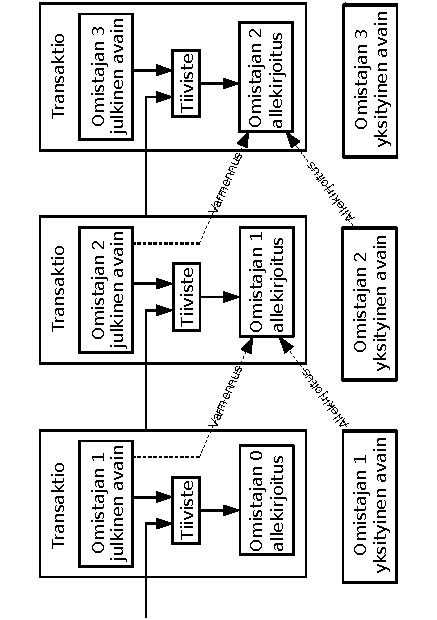
\includegraphics[angle=270,width=8.5cm]{figures/fig1.pdf}
\end{figure}

Ongelmaksi muodostuu tietenkin se, ettei maksunsaaja voi mitenkään tarkistaa, onko joku omistajista käyttänyt kolikon kahteen kertaan. Tavallinen ratkaisu on ottaa mukaan luotettu keskitetty auktoriteetti, toisin sanoen rahapaja, joka tarkistaa jokaisen transaktion \glsdisp{doublespend}{kaksin}kertaisen kulutuksen varalta. Jokaisen tapahtuman jälkeen kolikko on palautettava rahapajaan, joka laskee liikkeelle uuden kolikon, ja vain suoraan rahapajasta liikkeelle laskettujen kolikoiden voi luottaa olevan sellaisia, joita ei ole käytetty kahteen kertaan. Kuten pankkitoiminnassa, tämän ratkaisun ongelmana on koko rahajärjestelmän riippuvaisuus sitä ylläpitävästä yrityksestä, jonka kautta jokaisen siirron on kuljettava.

Tarvitsemme keinon, jolla maksunsaaja voi saada tietää, etteivät e\-del\-li\-set  omistajat ole allekirjoittaneet aiempia transaktioita. Tarkoitusperämme huomioiden vain varhaisimmalla siirrolla on merkitystä, joten emme välitä myö\-hem\-mis\-tä \glsdisp{doublespend}{kaksin}kertaisen kulutuksen yrityksistä. Vain olemalla tietoinen kaikista siirtotapahtumista voi vahvistaa tietyn siirron puuttumisen. Rahapajapohjaisessa mallissa rahapaja on tietoinen kaikista siirroista ja päättää, mikä niistä ovat tulleet ensimmäisenä perille. Jotta tämä voitaisiin suorittaa ilman luotettua kolmatta osapuolta, transaktioiden täytyy olla julkisia \cite{1} ja tarvitaan menetelmä, jonka avulla osallistujat pääsevät sopuun yhdestä ja samasta historiasta sille, missä järjestyksessä siirrot on vastaanotettu. Maksunsaaja tarvitsee todisteen siitä, että kunkin transaktion tapahtumahetkellä kyseinen transaktio oli solmujen enemmistön mielestä vastaanotettu ensimmäisenä.

\section{Aikaleimapalvelin}

Ehdottamamme ratkaisu alkaa \glsdisp{timestamp}aikaleimapalvelimesta. Aikaleimapalvelin toimii siten, että palvelimelle syötetään erinäisiä kirjauksia sisältävien lohkojen \glsdisp{hash}tiivisteitä, jotka palvelin aikaleimaa ja julkaisee laajasti – niin kuin sanomalehti tai Usenet-viesti [2–5]\vphantom{\cite{2}\cite{3}\cite{4}\cite{5}}. Aikaleima todistaa, että päätyäkseen mukaan tiivisteeseen tietojen on luonnollisesti täytynyt kyseisellä hetkellä olla olemassa. Jokaisen aikaleiman tiivisteeseen sisältyy aina edellinen \glsdisp{timestamp}aikaleima, mistä muodostuu ketju, jossa jokainen uusi aikaleima vahvistaa sitä edeltäneitä aikaleimoja.

\begin{figure}[H]
    \centering
    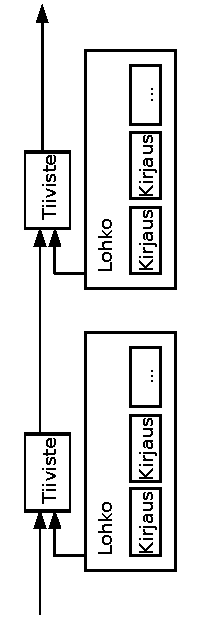
\includegraphics[angle=270,width=\textwidth]{figures/fig2.pdf}
\end{figure}

\section{Työntodiste}

Hajautetun \glsdisp{timestamp}aikaleimapalvelimen toteuttamiseksi \glsdisp{p2p}{vertais}verkossa vaaditaan työn\-to\-dis\-te\-jär\-jes\-tel\-mä, joka muistuttaa Adam Backin Hashcash-järjestelmää \cite{6} sanomalehden tai Usenet-viestien sijaan. Työntodistelaskennassa etsitään sellaista arvoa, jonka \glsdisp{hash}tiiviste esimerkiksi SHA-256-algoritmilla tiivistelaskettuna alkaa joukolla nollabittejä. Keskimääräisesti tämän arvon etsiminen vaatii vaadittujen nollabittien määrään nähden eksponentiaalisesti työtä, ja tehty työ voidaan varmentaa yhdellä  tiivistelaskelmalla.

Tässä ai\-ka\-lei\-ma\-ver\-kos\-sa työn\-to\-dis\-te\-jär\-jes\-tel\-mä toteutetaan lisäämällä lohkoon \glsdisp{nonce}nons\-se\-ja  eli kertakäyttöisiä arvoja niin kauan, kunnes löydetään sellainen arvo, joka tuottaa loh\-kon tiivisteeseen vaaditun määrän nollabittejä. Kun \glsdisp{tyontodiste}työn\-to\-dis\-teen vaatimukset täyttävä määrä prosessointitehoa on kerran kulutettu, ei lohkoa voi muuttaa laskematta työntodistetta uudelleen. Koska lohkot on ketjutettu toisiinsa, yhtäkään lohkoa ei voi muuttaa laskematta myös kaikkia sen jälkeen tulevia lohkoja uudelleen.

\begin{figure}[H]
    \centering
    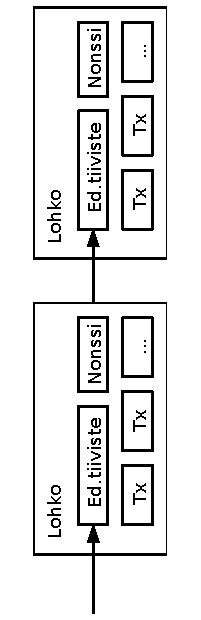
\includegraphics[angle=270,width=\textwidth]{figures/fig3.pdf}
\end{figure}

Työntodisteella ratkaistaan myös edustuksen määräytymiseen liittyvät ongelmat enemmistöpäätöksiä tehtäessä. Jos \glsdisp{ip}IP-osoite määrittäisi äänioikeuden, voisi useita IP-osoitteita itselleen varaamalla vääristää ää\-nes\-tys\-tu\-lok\-si\-a . Työn\-to\-dis\-te\-jär\-jes\-tel\-mäs\-sä  käytännössä jokaisella prosessorilla on yksi ääni. Tällöin pisin ketju, jonka \glsdisp{tyontodiste}työntodisteisiin on sijoitettu eniten vaivaa, edustaa e\-nem\-mis\-tö\-pää\-tös\-tä. Jos vilpittömät solmut hallitsevat suurinta osaa prosessointitehosta, vilpitön ketju kasvaa nopeimmin ja päihittää kilpailevat ketjut. Muokatakseen jotakin aiemmista lohkoista hyökkääjän täytyisi laskea paitsi kyseisen lohkon myös kaikkien sen jälkeen tulleiden lohkojen työntodisteet uudelleen ja sen jälkeen vielä saada vilpittömien solmujen tekemä työmäärä kiinni ja ylittää se. Osoitamme myöhemmin, miten todennäköisyys sille, että hitaampi hyökkääjä saisi vilpittömän ketjun kiinni, pienenee eksponentiaalisesti jokaisen lisätyn lohkon myötä.

Aikojen saatossa laitteistojen nopeudet kasvavat ja kiinnostus solmujen ajamista kohtaan vaihtelee. Tätä kompensoidaan säätämällä \glsdisp{tyontodiste}{työnt}odisteen laskennan keskimääräistä vaikeutta aina sen mukaan, kuinka paljon lohkoja keskimäärin tunnissa syntyy. Jos niitä syntyy liian nopeasti, vaikeus kasvaa.

\section{Verkko}

Verkon toiminta voidaan jakaa seuraaviin vaiheisiin:

\begin{enumerate}
    \item Uudet tapahtumat lähetetään kaikille solmuille.
    \item Jokainen solmu kerää uusia tapahtumia lohkoon.
    \item Jokainen solmu pyrkii löytämään vaikean \glsdisp{tyontodiste}{työnt}odisteen lohkolleen.
    \item Kun solmu löytää työntodisteen, se lähettää lohkonsa kaikille solmuille.
    \item Solmut hyväksyvät lohkon vain, jos kaikki sen sisältämät siirrot ovat kelvollisia eikä niitä ole jo kertaalleen käytetty.
    \item Solmut ilmaisevat hyväksyvänsä lohkon alkamalla työstää ketjun seuraavaa lohkoa hyväksytyn lohkon \glsdisp{hash}tiivisteen päälle.
\end{enumerate}

Solmut pitävät pisintä ketjua aina oikeana ja jatkavat työskentelyä sen pidentämisen parissa. Jos kaksi solmua lähettää samaan aikaan eri version seuraavasta lohkosta, osa solmuista saattaa vastaanottaa ne eri järjestyksessä. Siinä tapauksessa ne työstävät sitä haaraa, jonka vastaanottivat ensimmäisenä, mutta tallentavat toisen haaran siltä varalta, että siitä tulee pidempi. Tasapeli ratkeaa, kun seuraava \glsdisp{tyontodiste}{työnt}odiste löytyy ja toisesta haarasta tulee pidempi. Toista haaraa työstäneet solmut siirtyvät silloin pidemmän haaran pariin.

Uusien transaktioiden lähetysten ei tarvitse välttämättä tavoittaa kaikkia solmuja. Kunhan ne tavoittavat monia solmuja, ne ennen pitkää päätyvät johonkin lohkoon. Lohkojen lähetyksessä siedetään myös pudonneita viestejä. Jos jokin solmuista ei vastaanota tiettyä lohkoa, se pyytää sitä seuraavan lohkon vastaanottamisen yhteydessä havaitessaan jääneensä yhtä vaille.


\section{Kannustin}

Verkossa on käytäntönä pitää aina lohkon ensimmäistä siirtotapahtumaa erityisenä: se luo uuden kolikon, jonka omistaa lohkon luoja. Tämä antaa solmuille lisäkannustimen tukea verkkoa ja toimii keinona laskea kolikoita liikkeelle ilman keskitettyä liikkeelle laskevaa viranomaista. Uusia kolikoita tulee tasaisesti lisää vakiomäärä samaan tapaan kuin kultaa tulee kiertoon lisää kullankaivajien kuluttaessa resurssejaan. Meidän tapauksessamme kulutetaan prosessoriaikaa ja sähköä.

Kannustin voidaan rahoittaa myös siirtomaksuilla. Mikäli siirtotapahtuman tulosarvo on pienempi kuin sen syötearvo, niiden välinen erotus on siirtomaksu, joka lisätään sen lohkon kannustinarvoon, johon kyseinen siirtotapahtuma sisältyy. Heti kun ennalta määritelty määrä kolikoita on tullut kiertoon, kannustin voi kokonaisuudessaan muodostua siirtomaksuista ja olla täysin vapaa inflaatiosta.

Kannustin voi osaltaan auttaa pitämään solmut vilpittöminä. Jos ahne hyök\-kää\-jä  kykenee kokoamaan enemmän prosessointitehoa kuin kaikki vilpittömät solmut yhteensä, hänen täytyisi valita sen välillä, huijaako ihmisiä anastaakseen tekemänsä maksut takaisin itselleen vai tuottaako uusia kolikoita. Hänen luulisi pitävän kannattavampana vaihtoehtona pelata sellaisten sääntöjen mukaan, jotka suosivat häntä suoden hänelle enemmän uusia kolikoita kuin muille yhteensä, kuin sabotoida koko järjestelmää ja samalla heikentää oman varallisuutensa arvoa.

\section{Levytilan uusiokäyttö}

Kun kolikon viimeisin transaktio on hautautunut riittävän monen lohkon alle, ennen sitä tehdyt, kertaalleen käytetyt transaktiot voidaan levytilan sääs\-tä\-mi\-sek\-si poistaa. Jotta tämä voisi tapahtua rikkomatta lohkon \glsdisp{hash}tiivistettä, transaktiot on hajautettu Merkle-puuhun \cite{7}\cite{2}\cite{5}, josta pelkkä juuri on sisällytetty lohkon tiivisteeseen. Vanhempia lohkoja voidaan sitten pakata tiiviimpään muotoon puun haaroja katkaisemalla. Lohkon sisällä olevia tiivisteitä ei tarvitse säilyttää.

\begin{figure}[H]
    \centering
    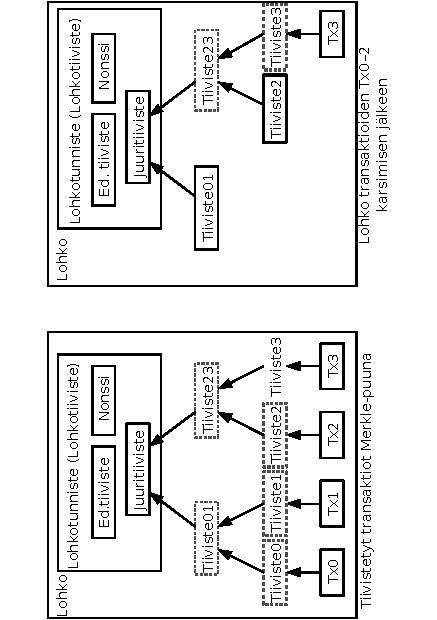
\includegraphics[angle=270,width=\textwidth]{figures/fig4.pdf}
\end{figure}

Lohkon tunniste ilman transaktioita on kooltaan noin 80 tavua. Jos oletamme, että lohkoja syntyy 10 minuutin välein, 80 tavua * 6 * 24 * 365 = 4,2 Mt vuodessa. Koska vuonna 2008 myytyihin tietokonejärjestelmiin sisältyi tyypillisesti 2 Gt RAM-muistia ja Mooren laki ennustaa tietokoneiden muistikapasiteetin kasvavan näillä näkymin 1,2 Gt vuodessa, tallennustilan ei pitäisi muodostua ongelmaksi, vaikka lohkon tunnisteet olisikin säilytettävä muistissa.

\section{Yksinkertaistettu maksunvarmennus}

Maksut on mahdollista varmentaa ajamatta täyttä verkkosolmua. Käyttäjän tarvitsee ainoastaan säilyttää kopio lohkon tunnisteista siitä \glsdisp{tyontodiste}{työnt}odisteketjusta, jonka on vakuuttunut olevan pisin muille verkkosolmuille tekemiensä kyselyjen perusteella, sekä löytää se Merkle-puun haara, joka linkittää kyseisen transaktion siihen lohkoon, johon se on \glsdisp{timestamp}aikaleimattu. Käyttäjä ei pysty varmistamaan siirtotapahtumaansa itse, mutta linkittämällä sen tiettyyn kohtaan ketjussa hän havaitsee, kun jokin verkon solmuista on kelpuuttanut sen, ja kyseisen siirron jälkeen lisätyt lohkot toimivat vahvistuksena siitä, että koko verkkokin on kelpuuttanut sen.

\begin{figure}[H]
    \centering
    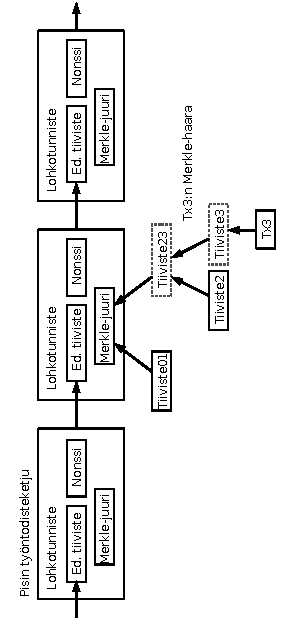
\includegraphics[angle=270,width=\textwidth]{figures/fig5.pdf}
\end{figure}

Varmennus on sinänsä luotettava, mutta vain niin kauan kuin vil\-pit\-tö\-mät solmut hallitsevat verkkoa; hyökkääjän onnistuessa valtaamaan verkon varmennuksesta tulee haavoittuvaisempi. Verkkosolmut pystyvät varmentamaan toistensa siirtotapahtumia, mutta hyökkääjä kykenee huijaamaan yksinkertaistettua menetelmää väärennetyillä siirroillaan niin kauan kuin pitää verkkoa vallassaan. Yksi tapa suojautua tältä olisi ottaa käyttöön hälytykset, joita verkkosolmut antaisivat epäkelpoja lohkoja havaitessaan. Hälytykset toimisivat kehotteena käyttäjän ohjelmistolle ladata koko lohko ja hälytyksiä aiheuttaneet siirrot ristiriitaisuuksien vahvistamiseksi. Yritykset, joiden maksuliikenne on vilkasta, haluavat luultavasti silti ajaa omia solmujaan, jotta niiden turvallisuus olisi riippumattomampaa ja varmennukset nopeampia.
\newpage
\section{Arvon jakaminen ja yhdistäminen}

Vaikka jokaisesta siirretystä sentistä olisi mahdollista tehdä oma tapahtumansa, olisi niiden käsittely erillisinä kolikkoina kömpelöä. Jotta arvon jakaminen ja yhdistäminen olisi mahdollista, transaktiot koostuvat useista syöte- ja tulosarvoista. Normaalisti ne koostuvat joko yhdestä edellisen, suuremman tapahtuman syötteestä tai useista pienempiä summia yhdistävistä syötteistä sisältäen enintään kaksi tulosarvoa: toinen on itse maksu ja toinen lähettäjälle palautuvat mahdolliset vaihtorahat.

\begin{figure}[H]
    \centering
    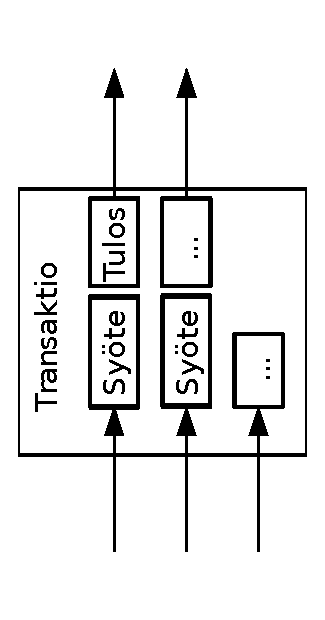
\includegraphics[angle=270,width=5cm]{figures/fig6.pdf}
\end{figure}

Huomautettakoon, että siirtojen \glsdisp{fanout}levittäytymisestä laajalle ("fan-out") eli siitä, että siirrot ovat riippuvaisia useista siirroista jotka puolestaan ovat riippuvaisia useista lisää, ei tässä synny ongelmaa. Koskaan ei tule tarvetta ottaa erillistä, täydellistä kopiota tietyn transaktion koko historiasta.

\section{Yksityisyys}

Pankkitoiminnan perinteisessä mallissa tietoihin pääsy on rajattu siten, että ainoastaan siirtotapahtuman osapuolet sekä luotettu kolmas osapuoli pääsevät niihin käsiksi, mikä luo jonkin verran yksityisyyttä. Kun kaikkien siirtojen on välttämätöntä olla julkisia, tällainen menetelmä on poissuljettu. Yksityisyyttä pystytään kuitenkin ylläpitämään katkaisemalla tiedonkulku toisesta kohtaa pitämällä julkiset \glsdisp{privatepublickey}avaimet nimettöminä. Kun joku lähettää jonkin summan jollekulle toiselle, siirto on kaikkien nähtävissä mutta ilman tietoja, jotka yhdistäisivät tapahtuman johonkin tiettyyn tahoon. Tämä on verrattavissa siihen, millaisia tietoja pörssit julkaisevat: yksittäisestä kaupasta kirjataan julkiselle "nauhalle" aika ja suuruus ilmoittamatta, keitä sen osapuolet olivat.

\begin{figure}[H]
    \centering
    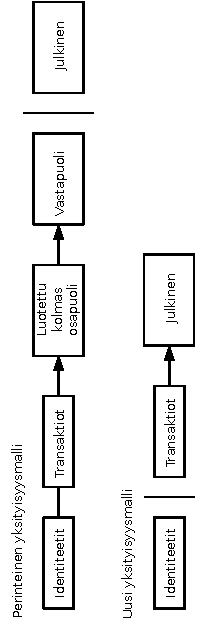
\includegraphics[angle=270,width=\textwidth]{figures/fig7.pdf}
\end{figure}

Jokaisessa transaktiossa tulisi käyttää lisäpalomuurina uutta avainparia, jotta tapahtumia ei voi yhdistää yhteiseen omistajaan. Tältä ei kuitenkaan voi täysin välttyä useamman syötteen siirroissa, joista pakostakin ilmenee syöt\-tei\-den olleen samassa omistuksessa. Tähän liittyy se riski, että jos tietyn \glsdisp{privatepublickey}avaimen omistaja paljastuu, tietoja yhdistelemällä voisi paljastua muitakin samalle omistajalle kuuluvia transaktioita.

\section{Laskelmat}

Tarkastellaanpa skenaariota, jossa hyökkääjä yrittää luoda vaihtoehtoisen ketjun vilpitöntä ketjua nopeammin. Vaikka hyökkääjän onnistuisi niin tehdä, koko järjestelmä ei yhtäkkiä olisi alttiina mielivaltaisille muutoksille, kuten että arvoa luotaisiin tyhjästä tai että hyökkääjä saisi anastettua rahaa, joka ei koskaan hänelle kuulunut. Solmut eivät kuitenkaan hyväksyisi epäkelpoja siirtoja maksuiksi, eivätkä vilpittömät solmut koskaan hyväksy lohkoja, joihin sisältyy epäkelpoja siirtoja. Hyökkääjä voi ainoastaan yrittää muuttaa yhtä omista transaktioistaan saadakseen takaisin rahat, jotka itse äskettäin käytti.

Vilpittömän ketjun ja hyökkääjäketjun välistä kilpailua voidaan luonnehtia \glsdisp{randomwalk}binominaaliseksi satunnaiskuluksi. Onnistuneeksi tapahtumaksi kutsutaan sitä, kun vilpitön ketju pitenee yhdellä lohkolla ja sen etumatka hyökkääjän ketjuun kasvaa (+1); epäonnistunut tapahtuma puolestaan on se, kun hyökkääjän ketju pitenee yhdellä lohkolla ja ketjujen välinen ero kaventuu (-1).

Hyökkääjän todennäköisyys saada kurottua välimatka umpeen altavastaaja-asemasta on vastaava kuin \glsdisp{gamblersruin}uhkapelurilla Gambler's Ruin -probleemassa. Oletetaan että uhkapelaaja, jolla on rajaton määrä pelirahaa, aloittaa tappiolla ja pelaa äärettömän monta peliä yrittäessään päästä omilleen. Todennäköisyys sille, että uhkapelaaja pääsee omilleen tai hyökkääjä kuroo umpeen välimatkan vilpittömään ketjuun, voidaan laskea seuraavasti \cite{8}:
\begin{itemize}
    \item[] $p =$ todennäköisyys sille, että vilpitön solmu löytää seuraavan lohkon
    \item[] $q =$ todennäköisyys sille, että hyökkääjä löytää seuraavan lohkon
    \item[] $q_{z} =$ todennäköisyys sille, että hyökkääjä koskaan kuroo umpeen $z$ lohkon etumatkan
\end{itemize}

\begin{equation*}
   q_{z} = 
   \begin{Bmatrix}
 1 & jos\quad p \leq q \\
  (q/p)^{z} & jos\quad p > q
 \end{Bmatrix}
\end{equation*}
\paragraph{}
Koska oletamme, että $p > q$, todennäköisyys pienenee eksponentiaalisesti sitä mukaa kun hyökkääjän kiinni kurottavien lohkojen määrä kasvaa. Todennäköisyydet eivät ole hänen puolellaan, joten jos hänen ei onnistu harpata ajoissa reilusti eteenpäin, hänen mahdollisuutensa kutistuvat häviävän pieniksi hänen jäädessään yhä kauemmas taakse.

Tarkastellaan seuraavaksi, kuinka kauan uuden siirron vastaanottajan on odotettava ennen kuin voi olla riittävän varma siitä, ettei lähettäjä pysty tekemään siirtoon muutoksia. Oletetaan, että lähettäjä on hyökkääjä, joka haluaa jonkin aikaa uskotella vastaanottajalle maksaneensa tälle mutta kääntääkin siirron jonkin ajan kuluttua takaisin itselleen. Vastaanottajalle ilmoitetaan, jos näin tapahtuu, mutta lähettäjä toivoo sen olevan liian myöhäistä.

Vastaanottaja luo uuden \glsdisp{privatepublickey}avainparin ja antaa julkisen avaimen lähettäjälle juuri ennen allekirjoitusta. Tällä estetään se, että lähettäjä voisi etukäteen valmistella lohkojen ketjua ja jatkuvasti työstää sitä siihen asti, kunnes hänen onnistuisi ottaa riittävästi etumatkaa, jolloin hän sitten suorittaisi siirtonsa. Kun siirto on lähetetty, epärehellinen lähettäjä alkaa salassa työstää rinnakkaisketjua, joka sisältää vaihtoehtoisen version hänen siirrostaan.

Vastaanottaja odottaa, kunnes tapahtuma on lisätty johonkin lohkoon ja $z$ määrä lohkoja on ketjutettu sen jälkeen. Hän ei tiedä tarkalleen, kuinka pitkälle hyökkääjä on edennyt, mutta kun oletetaan, että vilpittömiä lohkoja syntyy keskimääräisesti odotuksenmukaisella tahdilla, hyökkääjän edistyminen on \glsdisp{poissondistribution}Poisson-jakauma odotusarvolla:

\begin{equation*}
   \lambda = z \frac{q}{p}
\end{equation*}

\paragraph{} Jotta saadaan selville se todennäköisyys, jolla hyökkääjä vielä voisi kyseisellä hetkellä kuroa välimatkan umpeen, kerrotaan jokaisen mahdollisen siihenastisen edistysaskeleen Poisson-todennäköisyyden tiheys sillä todennäköisyydellä, jolla hän tuosta hetkestä käsin pystyisi ottamaan etumatkan kiinni:
\paragraph{}
\begin{equation*}
   {\sum_{k=0}^{\infty} \frac{\lambda^{k} e^{ - \lambda}}{k!}}\cdot
   \begin{Bmatrix}
 (q/p)^{(z - k)} & jos\quad k \leq z \\
  1 & jos\quad k > z
 \end{Bmatrix}
\end{equation*}

\paragraph{} Järjestellään tämä uudelleen niin, ettei jakauman ääretön häntä tule lasketuksi mukaan...

\begin{equation*}
   {1 - \sum_{k=0}^{z} \frac{\lambda^{k} e^{ - \lambda}}{k!}}
   \begin{pmatrix}1 - (q/p)^{(z - k)}
  \end{pmatrix}
\end{equation*}
\newpage
\noindent Muutetaan C-koodiksi...
\begin{verbatim}
#include <math.h>
double AttackerSuccessProbability(double q, int z)
{
    double p = 1.0 - q;
    double lambda = z * (q / p);
    double sum = 1.0;
    int i, k;
    for (k = 0; k <= z; k++)
    {
        double poisson = exp(-lambda);
        for (i = 1; i <= k; i++)
            poisson *= lambda / i;
        sum -= poisson * (1 - pow(q / p, z - k));
    }
    return sum;
}
\end{verbatim}

\noindent Laskemalla muutamia tuloksia voimme nähdä todennäköisyyden pienenevän $z$:lla eksponentiaalisesti:

\begin{verbatim}
q=0.1
z=0    P=1.0000000
z=1    P=0.2045873
z=2    P=0.0509779
z=3    P=0.0131722
z=4    P=0.0034552
z=5    P=0.0009137
z=6    P=0.0002428
z=7    P=0.0000647
z=8    P=0.0000173
z=9    P=0.0000046
z=10   P=0.0000012

q=0.3
z=0    P=1.0000000
z=5    P=0.1773523
z=10   P=0.0416605
z=15   P=0.0101008
z=20   P=0.0024804
z=25   P=0.0006132
z=30   P=0.0001522
z=35   P=0.0000379
z=40   P=0.0000095
z=45   P=0.0000024
z=50   P=0.0000006
\end{verbatim}

\noindent Ratkaistaan P-arvo alle 0,1 \%...

\begin{verbatim}
P < 0.001
q=0.10   z=5
q=0.15   z=8
q=0.20   z=11
q=0.25   z=15
q=0.30   z=24
q=0.35   z=41
q=0.40   z=89
q=0.45   z=340
\end{verbatim}

\section{Päätelmät}

Olemme esittäneet sähköisiin siirtoihin luottamuksesta riippumatonta jär\-jes\-tel\-mää. Lähdimme liikkeelle digitaalisista allekirjoituksista koostuvien kolikoiden tavanomaisesta viitekehyksestä: niiden omistusoikeuden hallinta on vahvaa, mutta ilman keinoja estää \glsdisp{doublespend}{kaksin}kertainen kulutus ne ovat vaillinaisia. Ratkaisuksi tähän esitimme \glsdisp{p2p}{vertais}verkkoa, jossa \glsdisp{tyontodiste}{työnt}odistejärjestelmän avulla siirtotapahtumat kirjataan julkiseen historiaan, jonka muuttamisesta tulee äkkiä hyökkääjälle laskennallisesti epäkäytännöllistä, mikäli prosessointitehosta suurin osa on vilpittömien solmujen hallussa. Verkko on kestävä kaikessa ohjaamattomassa yksinkertaisuudessaan. Solmut työskentelevät vähäisellä koordinaatiolla kaikki samaan aikaan. Solmujen ei tarvitse tunnistautua, sillä viestejä ei reititetä mihinkään tiettyyn paikkaan ja riittää, että verkko toimittaa viestit perille \glsdisp{besteffort}parhaansa mukaan. Solmut voivat poistua verkosta ja liittyä siihen milloin vain uudelleen, jolloin ne hyväksyvät \glsdisp{tyontodiste}{työnt}odisteketjun todisteeksi siitä, mitä tapahtui niiden poissa ollessa. Solmut äänestävät prosessointitehollaan ilmaisten hyväksyvänsä kelvolliset lohkot jatkamalla laskentaa niiden pohjalta ja hylkäävänsä epäkelvot lohkot kieltäytymällä rakentamasta niiden päälle. Kaikki tarvittavat säännöt ja kannustimet voidaan vahvistaa tällä \glsdisp{konsensus}konsensusmekanismilla.
\newpage
\printbibliography

\newpage

\section*{Suomentajilta}

Satoshi Nakamoto yhdistelee monien eri tieteenalojen käsitteitä. Tähän sanastoon on kerätty niistä keskeisimmät. Linkkien takaa löydät aiheesta lisätietoa suomeksi tai englanniksi, mikäli suomenkielistä materiaalia ei käännöshetkellä löytynyt. Anna palautetta suomennoksesta: \texttt{Biocycle@protonmail.com}, tai ota yhteyttä kääntäjiin Telegramin kautta.

\glsnogroupskiptrue
\printglossary

\end{document}